\subsection{Reconnaissance vocale de mots-clés}


\begin{frame}{La reconnaissance de mots-clés}
	\begin{block}{}
		\begin{description}
			\item[n°15] malaise, hémorragie, brûlure, intoxication
			\item[n°17] violences, agression, vol, cambriolage
			\item[n°18] incendie, gaz, effondrement, électrocution
		\end{description}
	\end{block}
	\begin{figure}
		\begin{subfigure}[]{0.31\textwidth}
			\includegraphics[width=\textwidth]{1-Incendie.jpg}
			\caption{INCENDIE}
		\end{subfigure}
		\begin{subfigure}[]{0.31\textwidth}
			\includegraphics[width=\textwidth]{1-Intoxication.jpg}
			\caption{INTOXICATION}
		\end{subfigure}
		\begin{subfigure}[]{0.31\textwidth}
			\includegraphics[width=\textwidth]{1-Cambriolage.jpg}
			\caption{CAMBRIOLAGE}
		\end{subfigure}
	\end{figure}
\end{frame}


\begin{frame}{La création de la base de données}
	\begin{columns}[T]
		\begin{column}[]{0.47\textwidth}
			\begin{exampleblock}{Données d'apprentissage : $6\times 12$}
				\begin{description}
					\item[Agathe]  $1\times12$ données
					\item[Florent]  $1\times12$ données
					\item[Tien-Thinh]  $4\times12$ données
				\end{description}
			\end{exampleblock}
		\end{column}
		\begin{column}[]{0.47\textwidth}
			\begin{alertblock}{Données d'évaluation : $3\times 12$}
				\begin{description}
					\item[Agathe]  $1\times12$ données
					\item[Florent]  $1\times12$ données
					\item[Tien-Thinh]  $1\times12$ données
				\end{description}
			\end{alertblock}
		\end{column}
	\end{columns}
	\begin{block}{Problématiques}
		\begin{itemize}
			\item Les spectrogrammes sont trop grands, de tailles 374*129
			\item Trop peu de données pour la rétropropagation
		\end{itemize}
	\end{block}
\end{frame}


\begin{frame}{L'augmentation de données}
	\begin{columns}[]
		\begin{column}[]{0.6\textwidth}
			\begin{block}{L'augmentation de données}
				Création de nouvelles données à partir des données existantes :
				\begin{itemize}
					\item Variation de ton
					\item Variation de vitesse
					\item Décalage temporel
					\item Ajout de bruit
				\end{itemize}
			\end{block}
			\begin{figure}
				\includegraphics[width=\textwidth]{7-origine.jpg}
			\end{figure}
		\end{column}
		\begin{column}[]{0.4\textwidth}
			\includegraphics[height=0.2\textheight]{7-pitch.jpg}
			\includegraphics[height=0.2\textheight]{7-speed.jpg}
			\includegraphics[height=0.2\textheight]{7-shift.jpg}
			\includegraphics[height=0.2\textheight]{7-noise.jpg}

		\end{column}
	\end{columns}
\end{frame}


\begin{frame}{Le transfert d'apprentissage à partir d'un réseau modèle}
	\begin{block}{Le réseau de neurones modèle, juste à $84\%$}
		Il est entrainé sur 8 000 données pour reconnaitre les $8$ mots : \\
		$["no",\ "stop",\ "up",\ "right",\ "yes",\ "left",\ "go",\ "down"]$ \\
	\end{block}
	\begin{exampleblock}{L'adaptation}
		\begin{itemize}
			\item La durée des audios est différente
			\item Le nombre de sorties est différent
		\end{itemize}
	\end{exampleblock}
\end{frame}



\begin{frame}{Un schéma du transfert d'apprentissage}
	\begin{figure}
		\includegraphics[width=\textwidth]{2-transfert.png}
		\caption{Schéma de fonctionnement du transfert d'apprentissage}
	\end{figure}
\end{frame}


\begin{frame}{Mes résultats}
	\begin{figure}
		\begin{subfigure}[]{0.49\textwidth}
			\includegraphics[width=\textwidth]{4-loss.jpg}
			\caption{Erreur au cours de l'apprentissage}
		\end{subfigure}
		\begin{subfigure}[]{0.49\textwidth}
			\includegraphics[width=\textwidth]{4-accuracy.jpg}
			\caption{Taux de bonnes réponses}
		\end{subfigure}
	\end{figure}
	\begin{columns}[T]
		\begin{column}{0.25\textwidth}
		\end{column}
		\begin{column}[]{0.50\textwidth}
			\begin{block}{Précision finale}
				\begin{description}
					\item[Agathe]  $50\%$ accuracy
					\item[Florent]  $75\%$ accuracy
					\item[Tien-Thinh]  $75\%$ accuracy
				\end{description}
			\end{block}
		\end{column}
		\begin{column}{0.25\textwidth}
		\end{column}
	\end{columns}
\end{frame}



\begin{frame}{Conclusion : Schéma de la réalisation du réseau de neurones}
	\begin{figure}
		\centering
		\includegraphics[height=0.7\textheight]{6-schema.png}
		\caption{Structure de mon réseau de neurones}
	\end{figure}
\end{frame}


\begin{frame}{Conclusion : Les moteurs de reconnaissance vocale}
	\begin{figure}
		\begin{center}
			\centering
			\includegraphics[width=0.4\textwidth]{3-incendie.png}
			\caption{Analyse du mot "INCENDIE"}
		\end{center}
	\end{figure}

	\begin{exampleblock}{Les performances moyennes des moteurs de reconnaissance vocale}
		\begin{itemize}
			\item Textes lus (dictée vocale, système monolocuteur) : 95 \%
			\item Journaux radio et TV : 90 \%
			\item Conversations téléphoniques informelles : 60 \%
		\end{itemize}
	\end{exampleblock}
\end{frame}